\documentclass[a4paper,12pt]{article}
\usepackage[T2A]{fontenc}
\usepackage[utf8]{inputenc}
\usepackage[russian]{babel}
\usepackage{amsmath, amssymb}
\usepackage{setspace}
\usepackage[left=2cm, right=2cm, top=2cm, bottom=2cm]{geometry}
\usepackage{graphicx}
\usepackage{listings}
\usepackage{xcolor} % Для подсветки
\usepackage{float} 

\begin{document}

\setcounter{page}{1}
\setstretch{1.0}
\thispagestyle{empty}
\newgeometry{
	left=0mm,
    top=20mm,
    right=0mm,
    bottom=20mm
}
\begin{center}
\bf
\vspace{4cm}
{
\setstretch{0.9}
\mbox{МИНИСТЕРСТВО~ОБРАЗОВАНИЯ~РЕСПУБЛИКИ~БЕЛАРУСЬ} \\~\\
\mbox{БЕЛОРУССКИЙ~ГОСУДАРСТВЕННЫЙ~УНИВЕРСИТЕТ} \\~\\
\mbox{ФАКУЛЬТЕТ ПРИКЛАДНОЙ МАТЕМАТИКИ И ИНФОРМАТИКИ} \\~\\
\mbox{Кафедра~биомедицинской~информатики} \\~\\
}
\vspace{4cm}
\bf
\mbox{Лабораторная работа 3}\\
\vspace{1cm}
\vspace{3cm}
\end{center}
\begin{tabular}{ll}
\hspace{10.5cm}
&Снежко Льва Владимировича~\\
&студента 3-го курса\\~\\
&Преподаватель:\\
&Дайняк Виктор Владимирович
\end{tabular}
\vspace{7cm}
\begin{center}
Mинск, 2025
\end{center}
\clearpage
\restoregeometry
\title{Вариант 12}
\date{}
\maketitle

\section{Задача 1}

\[
\quad
\begin{cases}
u_{tt} = a^2 u_{xx} + g \\
u|_{x=0} = 0 \\
u|_{x=\ell} = 0 \\
u|_{t=0} = 0, \quad u_t|_{t=0} = v
\end{cases}
\]

Обозначим: \( u = P \cdot Q \)

\[
\begin{cases}
P_{tt} = a^2 P_{xx} \\
P|_{x=0} = 0 \\
P|_{x=\ell} = 0 \\
P|_{t=0} = 0, \quad P_t|_{t=0} = v
\end{cases}
\]

Предположим: \( P = T \cdot X \)

\[
T'' X = a^2 T X''
\Rightarrow
\frac{T''}{a^2 T} = \frac{X''}{X} = -\lambda
\]

\[
X'' + \lambda X = 0 \Rightarrow X = C_1 \cos \sqrt{\lambda} x + C_2 \sin \sqrt{\lambda} x
\]

\[
X(0) = 0 \Rightarrow C_1 = 0
\]

\[
X(\ell) = 0 \Rightarrow \sin(\sqrt{\lambda} \ell) = 0 \Rightarrow 
\sqrt{\lambda} = \frac{\pi + 2k\pi}{2\ell}
\]

\[
\boxed{
X_k = \sin\left( \frac{\pi + 2k\pi}{2\ell} x \right)
}
\]

\[
T_k = A_k \cos a \sqrt{\lambda_k} t + B_k \sin a \sqrt{\lambda_k} t
\]

\[
P = \sum_{k=1}^{\infty} \left( A_k \cos a \sqrt{\lambda_k} t + B_k \sin a \sqrt{\lambda_k} t \right) \sin\left( \frac{\pi + 2k\pi}{2\ell} x \right)
\]

Из начального условия:
\[
P|_{t=0} = \sum_{k=1}^{\infty} A_k \sin\left( \frac{\pi + 2k\pi}{2\ell} x \right) = 0 \quad \Rightarrow \quad A_k = 0,\quad k \in \mathbb{N}
\]

\[
P_t = \sum_{k=1}^{\infty} \left( B_k \cdot a \sqrt{\lambda_k} \cos\left( a \sqrt{\lambda_k} t \right) \cdot \sin\left( \frac{\pi + 2k\pi}{2\ell} x \right) \right)
\]

\[
P_t|_{t=0} = \sum_{k=1}^{\infty} B_k a \sqrt{\lambda_k} \sin\left( \frac{\pi + 2k\pi}{2\ell} x \right) = v
\]

Разложим \( v \) в ряд Фурье:

\[
v = \sum_{k=1}^{\infty} v_k \sin\left( \frac{\pi + 2k\pi}{2\ell} x \right)
\]

Имеем:
\[
\sum_{k=1}^{\infty} B_k a \sqrt{\lambda_k} \sin\left( \frac{\pi + 2k\pi}{2\ell} x \right) = \sum_{k=1}^{\infty} v_k \sin\left( \frac{\pi + 2k\pi}{2\ell} x \right)
\]

\[
\Rightarrow B_k = \frac{v_k}{a \sqrt{\lambda_k}} = \frac{v_k}{a \cdot \frac{\pi + 2k\pi}{2\ell}} = \frac{2\ell v_k}{a (\pi + 2k\pi)}
\]

Из разложения $v$ в ряд Фурье:
\[
v_k = \frac{4v}{\pi + 2k\pi}
\quad \Rightarrow \quad
B_k = \frac{8 v \ell}{(\pi + 2k\pi)^2 a}
\]

Подставим в общее решение:

\[
P = \sum_{k=1}^{\infty} \frac{8 v \ell}{(\pi + 2k\pi)^2 a} \sin\left( \frac{a (\pi + 2k\pi)}{2\ell} t \right) \sin\left( \frac{\pi + 2k\pi}{2\ell} x \right)
\]

Будем искать $Q$ в виде

\[
Q = T(t) \cdot X(x) = \sum_{k=1}^{\infty} T_k(t) \sin\left( \frac{\pi + 2k\pi}{2\ell} x \right)
\]

Исходное уравнение:
\[
Q_{tt} = a^2 Q_{xx} + g
\]

С начальными условиями:
\[
\begin{cases}
Q|_{t=0} = 0 \\
Q_t|_{t=0} = 0 \\
Q|_{x=0} = 0 \\
Q|_{x=2\ell} = 0
\end{cases}
\]

Подставим $Q$ в уравнение:

\[
\sum_{k=1}^{\infty} T_k''(t) \sin\left( \frac{\pi + 2k\pi}{2\ell} x \right) + a^2 \sum_{k=1}^{\infty} T_k(t) \left( \frac{\pi + 2k\pi}{2\ell} \right)^2 \sin\left( \frac{\pi + 2k\pi}{2\ell} x \right) = g
\]

Разложим $g$ в ряд Фурье:
\[
g = \sum_{k=1}^{\infty} \frac{4g}{\pi + 2k\pi} \sin\left( \frac{\pi + 2k\pi}{2\ell} x \right)
\]

Подставим:

\[
\sum_{k=1}^{\infty} \left( T_k''(t) + a^2 \left( \frac{\pi + 2k\pi}{2\ell} \right)^2 T_k(t) \right) \sin\left( \frac{\pi + 2k\pi}{2\ell} x \right)
= \sum_{k=1}^{\infty} \frac{4g}{\pi + 2k\pi} \sin\left( \frac{\pi + 2k\pi}{2\ell} x \right)
\]

Отсюда:
\[
\begin{cases}
T_k''(t) + a^2 \left( \frac{\pi + 2k\pi}{2\ell} \right)^2 T_k(t) = \frac{4g}{\pi + 2k\pi} \\
T_k(0) = 0 \\
T_k'(0) = 0
\end{cases}
\]

\textbf{Общее решение однородного:}
$$T_k = C_1 \cos a \sqrt{\lambda_k} t + C_2 \sin a \sqrt{\lambda_k} t$$

\textbf{Найдём общее решение неоднородного:}
$$C_1'(t) \cos a \sqrt{\lambda_k} t + C_2'(t) \sin a \sqrt{\lambda_k} t = 0$$
$$- C_1'(t) a \sqrt{\lambda_k} \sin a \sqrt{\lambda_k} t + C_2'(t) a \sqrt{\lambda_k} \cos a \sqrt{\lambda_k} t = \frac{4g}{\pi - 2xk}$$

$$\textbf{Выразим } C_1, C_2$$:
$$C_1(t) = \frac{16 g l^2}{a^2 (\pi + 2 x k)^3} \cos a \sqrt{\lambda_k} t$$
$$C_2(t) = \frac{16 g l^2}{a^2 (\pi + 2 x k)^3} \sin a \sqrt{\lambda_k} t$$

$$\textbf{Подставим и найдём } T_k:$$
$$T_k = \frac{16 g l^2}{a^2 (\pi + 2 x k)^3}$$

$$Q(x, t) = \sum_{k=1}^\infty \frac{16 g l^2}{a^2 (\pi + 2 x k)^3} \sin \frac{\pi - 2 x k}{2 l} x$$

$$u = P + Q = \sum_{k=1}^\infty \left( \frac{16 g l^2}{a^2 (\pi + 2 x k)^3} \sin \frac{a \sqrt{(\pi + 2 x k)^2}}{2 l} t \right) \sin \frac{\pi - 2 k}{2 l} x$$

\section{Задание 2}

$$\begin{cases}
u_{tt} = a^2 u_{xx} + \sin \frac{\pi x}{l} \sin \frac{\pi t}{l}, \quad 0 < x < l,\ t > 0 \\
u|_{x=0} = 0, \quad u|_{x=l} = 0 \\
u|_{t=0} = 2x \\
u_t|_{t=0} = 0
\end{cases}$$

\subsection*{Будем искать решение в виде $u = P + Q$}

$$\begin{cases}
P_{tt} = a^2 P_{xx} \\
P|_{x=0} = 0, \quad P|_{x=l} = 0 \\
P|_{t=0} = 2x \\
P_t|_{t=0} = 0
\end{cases}
\qquad
\begin{cases}
Q_{tt} = a^2 Q_{xx} + \sin \frac{\pi x}{l} \sin \frac{\pi t}{l} \\
Q|_{x=0} = 0, \quad Q|_{x=l} = 0 \\
Q|_{t=0} = 0 \\
Q_t|_{t=0} = 0
\end{cases}$$

\subsection*{Найдём $P$ в виде $P = T(t) X(x)$}

$$\frac{T''}{a^2 T} = \frac{X''}{X} = -\lambda$$

$$\begin{cases}
X = C_1 \cos \sqrt{\lambda} x + C_2 \sin \sqrt{\lambda} x \\
X|_{x=0} = 0 \Rightarrow C_1 = 0 \\
X|_{x=l} = 0 \Rightarrow \sqrt{\lambda} l = n \pi
\end{cases}$$

$$X|_{x=0} = 0 \Rightarrow C_1 = 0$$
$$X|_{x=l} = C_2 \sin \sqrt{\lambda} l = 0 \Rightarrow \sqrt{\lambda_k} = \frac{\pi k}{l}$$

$$X_k = \sin \frac{\pi k}{l} x$$

$$P = \sum_{k=1}^\infty T_k \sin \frac{\pi k}{l} x$$

$$P_{tt} - a^2 P_{xx} = \sum_{k=1}^\infty \left( T_k'' - \left( \frac{\pi k}{l} \right)^2 a^2 T_k \right) \sin \frac{\pi k}{l} x = 0$$

$$\sum_{k=1}^\infty X_k T_k|_{t=0} = 2x
\quad \text{и} \quad
\sum_{k=1}^\infty X_k T_k'|_{t=0} = 0$$

$$T_k = A_k \cos \frac{a \pi k}{l} t + B_k \sin \frac{a \pi k}{l} t$$

\textbf{Подставим в уравнение и упростим, получим:}
$$\left( -B_k \cdot \frac{a \pi k}{l} + B_k \cdot \frac{a \pi k}{l} \right) \sin \frac{\pi k}{l} x = 0 \Rightarrow B_k = 0$$

$$\sum_{k=1}^\infty T_k X_k = \sum_{k=1}^\infty A_k \cos \frac{a \pi k}{l} t \cdot \sin \frac{\pi k}{l} x = 2x$$

\subsection*{Разложим $2x$ в ряд Фурье:}

$$2x = \sum_{k=1}^\infty \frac{-2l \cos \pi k}{1 - \cos \pi k} \sin \frac{\pi k}{l} x$$

\subsection*{Подставим:}

$$T_k = A_k \cos \frac{a \pi k}{l} t + \sin \frac{\pi k}{l} t
\Rightarrow
\sum_{k=1}^\infty T_k X_k|_{t=0} = \sum_{k=1}^\infty A_k \sin \frac{\pi k}{l} x$$

$$A_k = \frac{-2l \cos \pi k}{1 - \cos \pi k}$$

$$P = \sum_{k=1}^\infty \frac{-2l \cos \pi k}{1 - \cos \pi k} \cos \frac{a \pi k}{l} t \cdot \sin \frac{\pi k}{l} x$$

\subsection*{Составим задачу для $Q$:}

$$\begin{cases}
Q_{tt} = a^2 Q_{xx} + \sin \frac{a \pi t}{l} \sin \frac{\pi x}{l} \\
Q|_{x=0} = 0, \quad Q|_{x=l} = 0 \\
Q|_{t=0} = 0, \quad Q_t|_{t=0} = 0
\end{cases}$$

\subsection*{Найдём решение в виде:}

$$Q = T(t) X(x) = \sum_{k=1}^\infty T_k \sin \frac{\pi k}{l} x$$

\subsection*{Подставим в уравнение:}

$$\sum_{k=1}^\infty \left( T_k'' + \left( \frac{a \pi k}{l} \right)^2 T_k \right) \sin \frac{\pi k}{l} x = \sin \frac{a \pi t}{l} \sin \frac{\pi x}{l}$$

\subsection*{Имеем:}

$$\begin{cases}
T_k'' + \left( \frac{a \pi k}{l} \right)^2 T_k = \sin \frac{a \pi t}{l}, \quad k = 1 \\
T_k'' + \left( \frac{a \pi k}{l} \right)^2 T_k = 0, \quad k \ne 1 \\
T_k|_{t=0} = 0 \\
T_k'|_{t=0} = 0
\end{cases}$$

\subsection*{Решение однородного:}

$$T_k = C_1 \cos \frac{a \pi t}{l} + C_2 \sin \frac{a \pi t}{l}$$

\subsection*{Найдём решение неоднородного в виде:}

$$T_k = C_1(t) \cos \frac{a \pi t}{l} + C_2(t) \sin \frac{a \pi t}{l}$$

\subsection*{Используем метод вариации произвольных постоянных}

$$C_1(t) \cos \frac{a \pi x}{e} + C_2(t) \sin \frac{a \pi x}{e} - C_1(t) \frac{a \pi}{e} \sin \frac{a \pi x}{e} + C_2(t) \frac{a \pi}{e} \cos \frac{a \pi x}{e} \cdot \frac{dz}{dt} = \sin \frac{a \pi x}{e}$$

$$\text{Выразим } C_1, C_2, \text{ подставим:}$$

$$T_1''^2 = \left(-\frac{lt}{2at} + \left(\frac{l}{2at}\right)^2 \sin \frac{2a\pi t}{e} \cos \frac{a\pi t}{e} - \left(\frac{l}{at}\right)^2 \cdot \frac{1}{2} \sin^3 \frac{a\pi t}{e} \right)$$

$$\text{Таким образом } Q:$$

$$Q'' = \left(-\frac{lt}{2at} + \left(\frac{l}{2at}\right)^2 \sin \frac{2a\pi t}{e} \cos \frac{a\pi t}{e} - \left(\frac{l}{at}\right)^2 \cdot \frac{1}{2} \sin^3 \frac{a\pi t}{e} \right)$$

$$\text{Подставим и найдём } u:$$

$$u(x,t) = \left(1 - \frac{lt}{2at} + \left(\frac{l}{2at}\right)^2 \sin \frac{2a\pi t}{e} \cos \frac{a\pi t}{e} - \left(\frac{l}{at}\right)^2 \cdot \frac{1}{2} \sin^3 \frac{a\pi t}{e} \right) \cdot \sin \frac{\pi x}{e} $$
$$+ \sum_{k=1}^{\infty} \left( -2 \cdot \frac{\cos kl}{k \cos kl} \cos \frac{a k \pi t}{e} + \sin \frac{kl}{e} x \right)$$

\section{Задание 3}
$$\left\{
\begin{aligned}
  u_{xx} &= f(x), \quad &x \in (0,1) \\
  u|_{t=0} &= 2, \\
  u|_{t=0} &= 0, \\
  u_x|_{x=0} &= t, \\
  u_x|_{x = l} = -1
\end{aligned}
\right.$$

$$u = v + \omega$$

$$\omega = \frac{-t-1}{l}x^2 + tx$$
$$
\begin{cases}
v_{tt} - v_{xx} = t^2 - \frac{t+1}{l} - x \\
v|_{t=0} = 2 + \frac{x^2}{l}, \\
v_t|_{t=0} = 0, \\
v_x|_{x=0} = 0, \\
v_x|_{x=l} = 0
\end{cases}
$$

Будем искать решение в виде: $v = TX$

$$T'' X = a^2 T X'' $$
$$\frac{T''}{a^2 T} = \frac{X''}{X} = -\lambda$$

$$X_k = C_1 \cos\sqrt{\lambda}x + C_2 \sin\sqrt{\lambda}x$$

$$X_k'|_{x = 0} = 0 \Rightarrow C_2 = 0$$

$$X_k'|_{x = \ell} = C_1 \sqrt{\lambda} \sin(\sqrt{\lambda} \ell) = 0 \Rightarrow \sin(\sqrt{\lambda} \ell) = 0 \Rightarrow \sqrt{\lambda_k} = \frac{\pi k}{\ell}$$

$$X_k = \cos\left( \frac{\pi k}{\ell} x \right)$$

$$P = \sum_{k=1}^{\infty} T_k \cos\left( \frac{\pi k}{\ell} x \right)$$

\textbf{Подставим:}
$$\sum_{k=1}^{\infty} \left( T_k'' + \left( \frac{\pi k}{\ell} \right)^2 T_k \right) \cos\left( \frac{\pi k}{\ell} x \right) = t^2 - \frac{t+1}{l} - x$$

\textbf{Разложим в ряд Фурье:}
$$t^2 - \frac{t+1}{l} - x = \sum_{k=1}^{\infty} T_k X_k = \sum_{k=1}^{\infty} \frac{2(1 - \cos k \ell)}{\pi k} \cos\left( \frac{\pi k}{\ell} x \right)$$

\textbf{Имеем:}
$$T_k'' + \left( \frac{\pi k}{\ell} \right)^2 T_k = \frac{2(1 - \cos(k \ell))}{\pi k}$$

\textbf{Разложим $\phi = 2 + \frac{x^2}{l}$ в ряд Фурье}
$$\phi = \sum_{k=1}^{\infty}\frac{2lcos(\pi k)}{(\pi k)^2}cos(\frac{\pi k}{l}x)$$
\textbf{Подставим в начальные условия:}
$$\sum_{k=1}^{\infty}T_k cos(\frac{\pi k}{l}x)|_{t=0} = \sum_{k=1}^{\infty}\frac{2lcos(\pi k)}{(\pi k)^2}cos(\frac{\pi k}{l}x)$$
\textbf{Отсюда имеем:}
$$T_k|_{t=0} = \frac{2l cos(\pi k)}{(\pi k)^2}$$
$$
\begin{cases}
    T_k'' + \frac{\pi k}{l}T_k = \frac{2(1 - \cos(k \ell))}{\pi k} \\
    T_k|_{t=0} = \frac{2l cos(\pi k)}{(\pi k)^2} \\
    T_k'|_{t=0} = 0
\end{cases}
$$
$$T_k = A_k cos(\frac{\pi kt}{l}) + B_k sin(\frac{\pi kt}{l})$$
$$T_k |_{t=0} = \frac{2l cos(\pi k)}{(\pi k)^2} \Rightarrow A_k = \frac{2l cos(\pi k)}{(\pi k)^2}$$
$$T_k' |_{t=0} = \frac{\pi k}{l}B_k = 0 \Rightarrow B_k = 0$$
\textbf{Таким образом:}
$$T_k = \frac{2l cos(\pi k)}{(\pi k)^2}cos(\frac{\pi k t}{l})$$
$$v = \sum_{k=1}^{\infty}X_k T_k = \sum_{k=1}^{\infty} \frac{2l cos(\pi k)}{(\pi k)^2}cos(\frac{\pi k t}{l})cos(\frac{\pi k x}{l})$$
$$u = \sum_{k=1}^{\infty}X_k T_k = \sum_{k=1}^{\infty} \frac{2l cos(\pi k)}{(\pi k)^2}cos(\frac{\pi k t}{l})cos(\frac{\pi k x}{l}) - \frac{t+1}{l}x^2 + tx$$

\section{Визуализация 1}
$$u(x,t) = \sum_{k=1}^\infty \left( \frac{16 g l^2}{a^2 (\pi + 2 x k)^3} \sin \frac{a \sqrt{(\pi + 2 x k)^2}}{2 l} t \right) \sin \frac{\pi - 2 k}{2 l} x$$
\textbf{Ниже приведен код на языке Python, который изображает график данной функции}
\begin{lstlisting}
import numpy as np
import matplotlib.pyplot as plt
from mpl_toolkits.mplot3d import Axes3D

g = 9.8
l = 1
a = 1

x = np.linspace(0, 2 * l, 200)
t = np.linspace(0, 5, 200)
X, T = np.meshgrid(x, t)

U = np.zeros_like(X)
for k in range(1, 101):
    coef = (16 * g * l**2) / (a**2 * (np.pi + 2*k)**3)
    omega_k = a * (np.pi + 2*k) / (2 * l)
    U += coef * np.sin(omega_k * T) * np.sin((np.pi - 2*k) * X / (2 * l))

fig = plt.figure(figsize=(12, 6))
ax = fig.add_subplot(111, projection='3d')
ax.plot_surface(X, T, U, cmap='viridis')

ax.set_title('u(x, t)')
ax.set_xlabel('x')
ax.set_ylabel('t')
ax.set_zlabel('u(x, t)')

plt.savefig("graph1.png", dpi=300)
plt.show()

\end{lstlisting}
\begin{figure}[H]
    \centering
    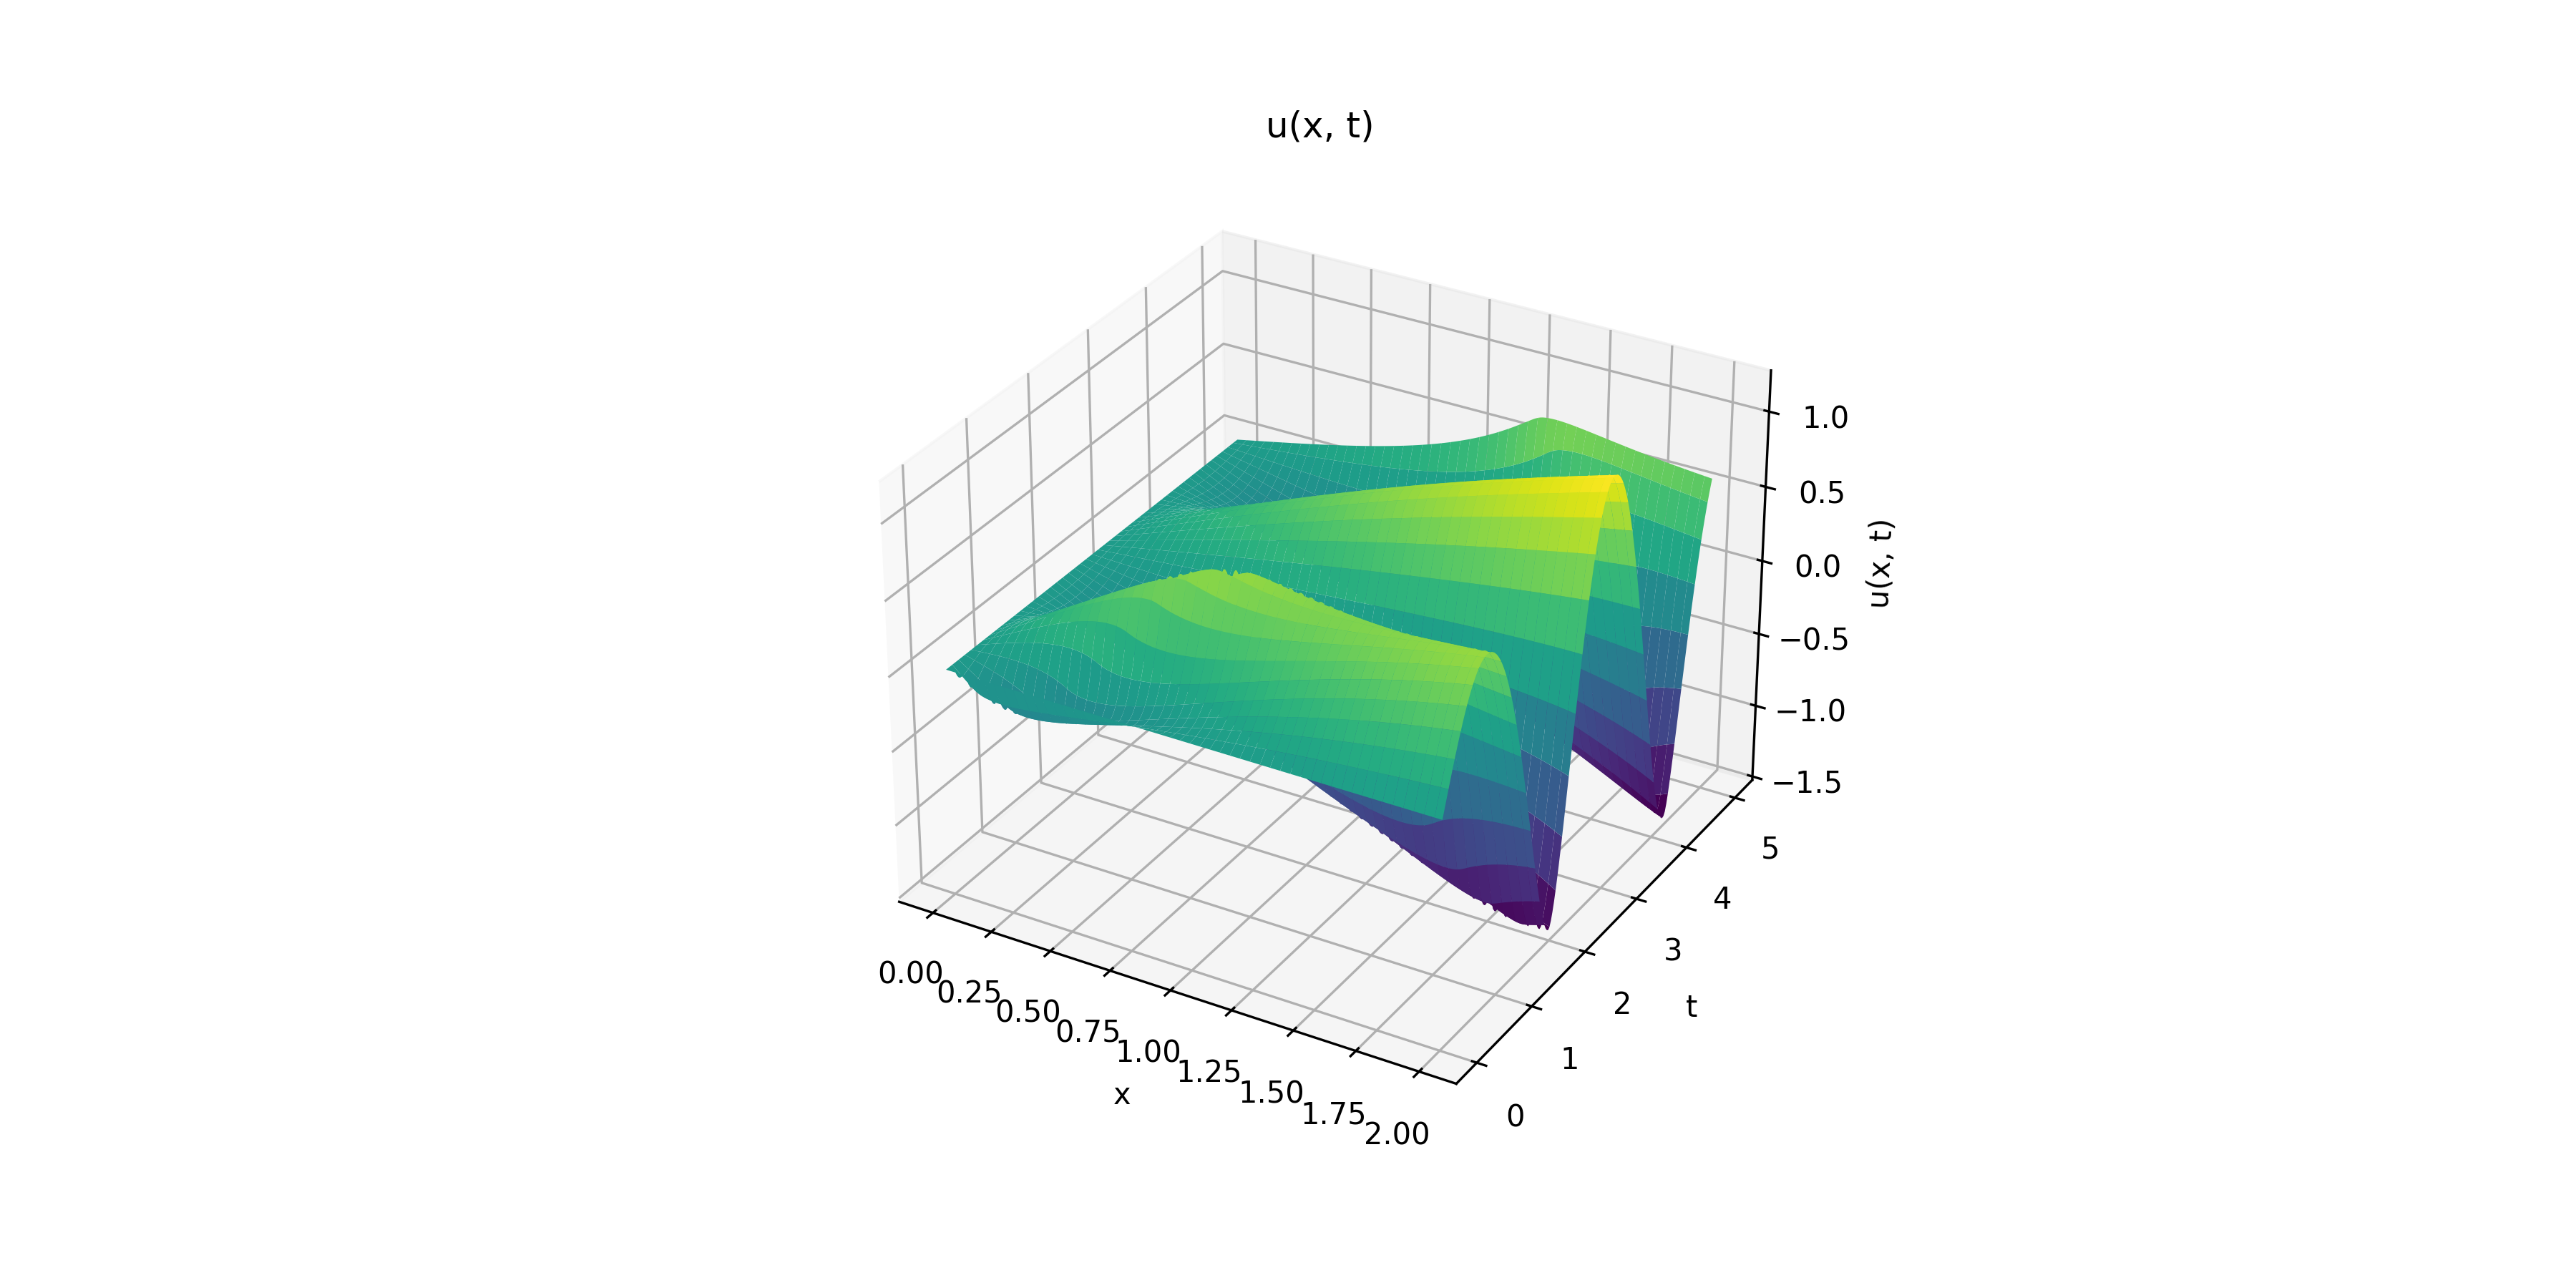
\includegraphics[width=0.8\textwidth]{../graph1.png}
    \caption{График функции $u(x,t)$, построенный по приближённой сумме ряда}

\end{figure}


\section{Визуализация 2}
$$u(x,t) = \left(1 - \frac{lt}{2at} + \left(\frac{l}{2at}\right)^2 \sin \frac{2a\pi t}{e} \cos \frac{a\pi t}{e} - \left(\frac{l}{at}\right)^2 \cdot \frac{1}{2} \sin^3 \frac{a\pi t}{e} \right) \cdot \sin \frac{\pi x}{e}$$
$$ + \sum_{k=1}^{\infty} \left( -2 \cdot \frac{\cos kl}{k \cos kl} \cos \frac{a k \pi t}{e} + \sin \frac{kl}{e} x \right)$$
\textbf{Ниже приведен код на языке Python, который изображает график данной функции}
\begin{lstlisting}
  import numpy as np
import matplotlib.pyplot as plt

from mpl_toolkits.mplot3d import Axes3D

a = 1
l = 1
e = 1
N = 100  
x = np.linspace(0, e, 200)
t = np.linspace(0.1, 5, 200)
X, T = np.meshgrid(x, t)

term1 = (1 - l / (2 * a) + ((l / (2 * a * T))**2) * np.sin(2 * a * np.pi * T / e) * np.cos(a * np.pi * T / e) -
         0.5 * (l / (a * T))**2 * np.sin(a * np.pi * T / e)**3) * np.sin(np.pi * X / e)

term2 = np.zeros_like(X)

for k in range(1, N + 1):
    denom = k * np.cos(k * l)
    if np.any(np.isclose(denom, 0)):
        continue
    term2 += (-2 * np.cos(k * l) / denom) * np.cos(a * k * np.pi * T / e) + np.sin((k * l / e) * X)

U = term1 + term2

fig = plt.figure(figsize=(12, 6))
ax = fig.add_subplot(111, projection='3d')
ax.plot_surface(X, T, U, cmap='plasma')

ax.set_title("u(x, t)")
ax.set_xlabel("x")
ax.set_ylabel("t")
ax.set_zlabel("u(x, t)")

plt.tight_layout()
plt.savefig("graph2.png", dpi=300)
plt.show()

\end{lstlisting}
\begin{figure}[H]
    \centering
    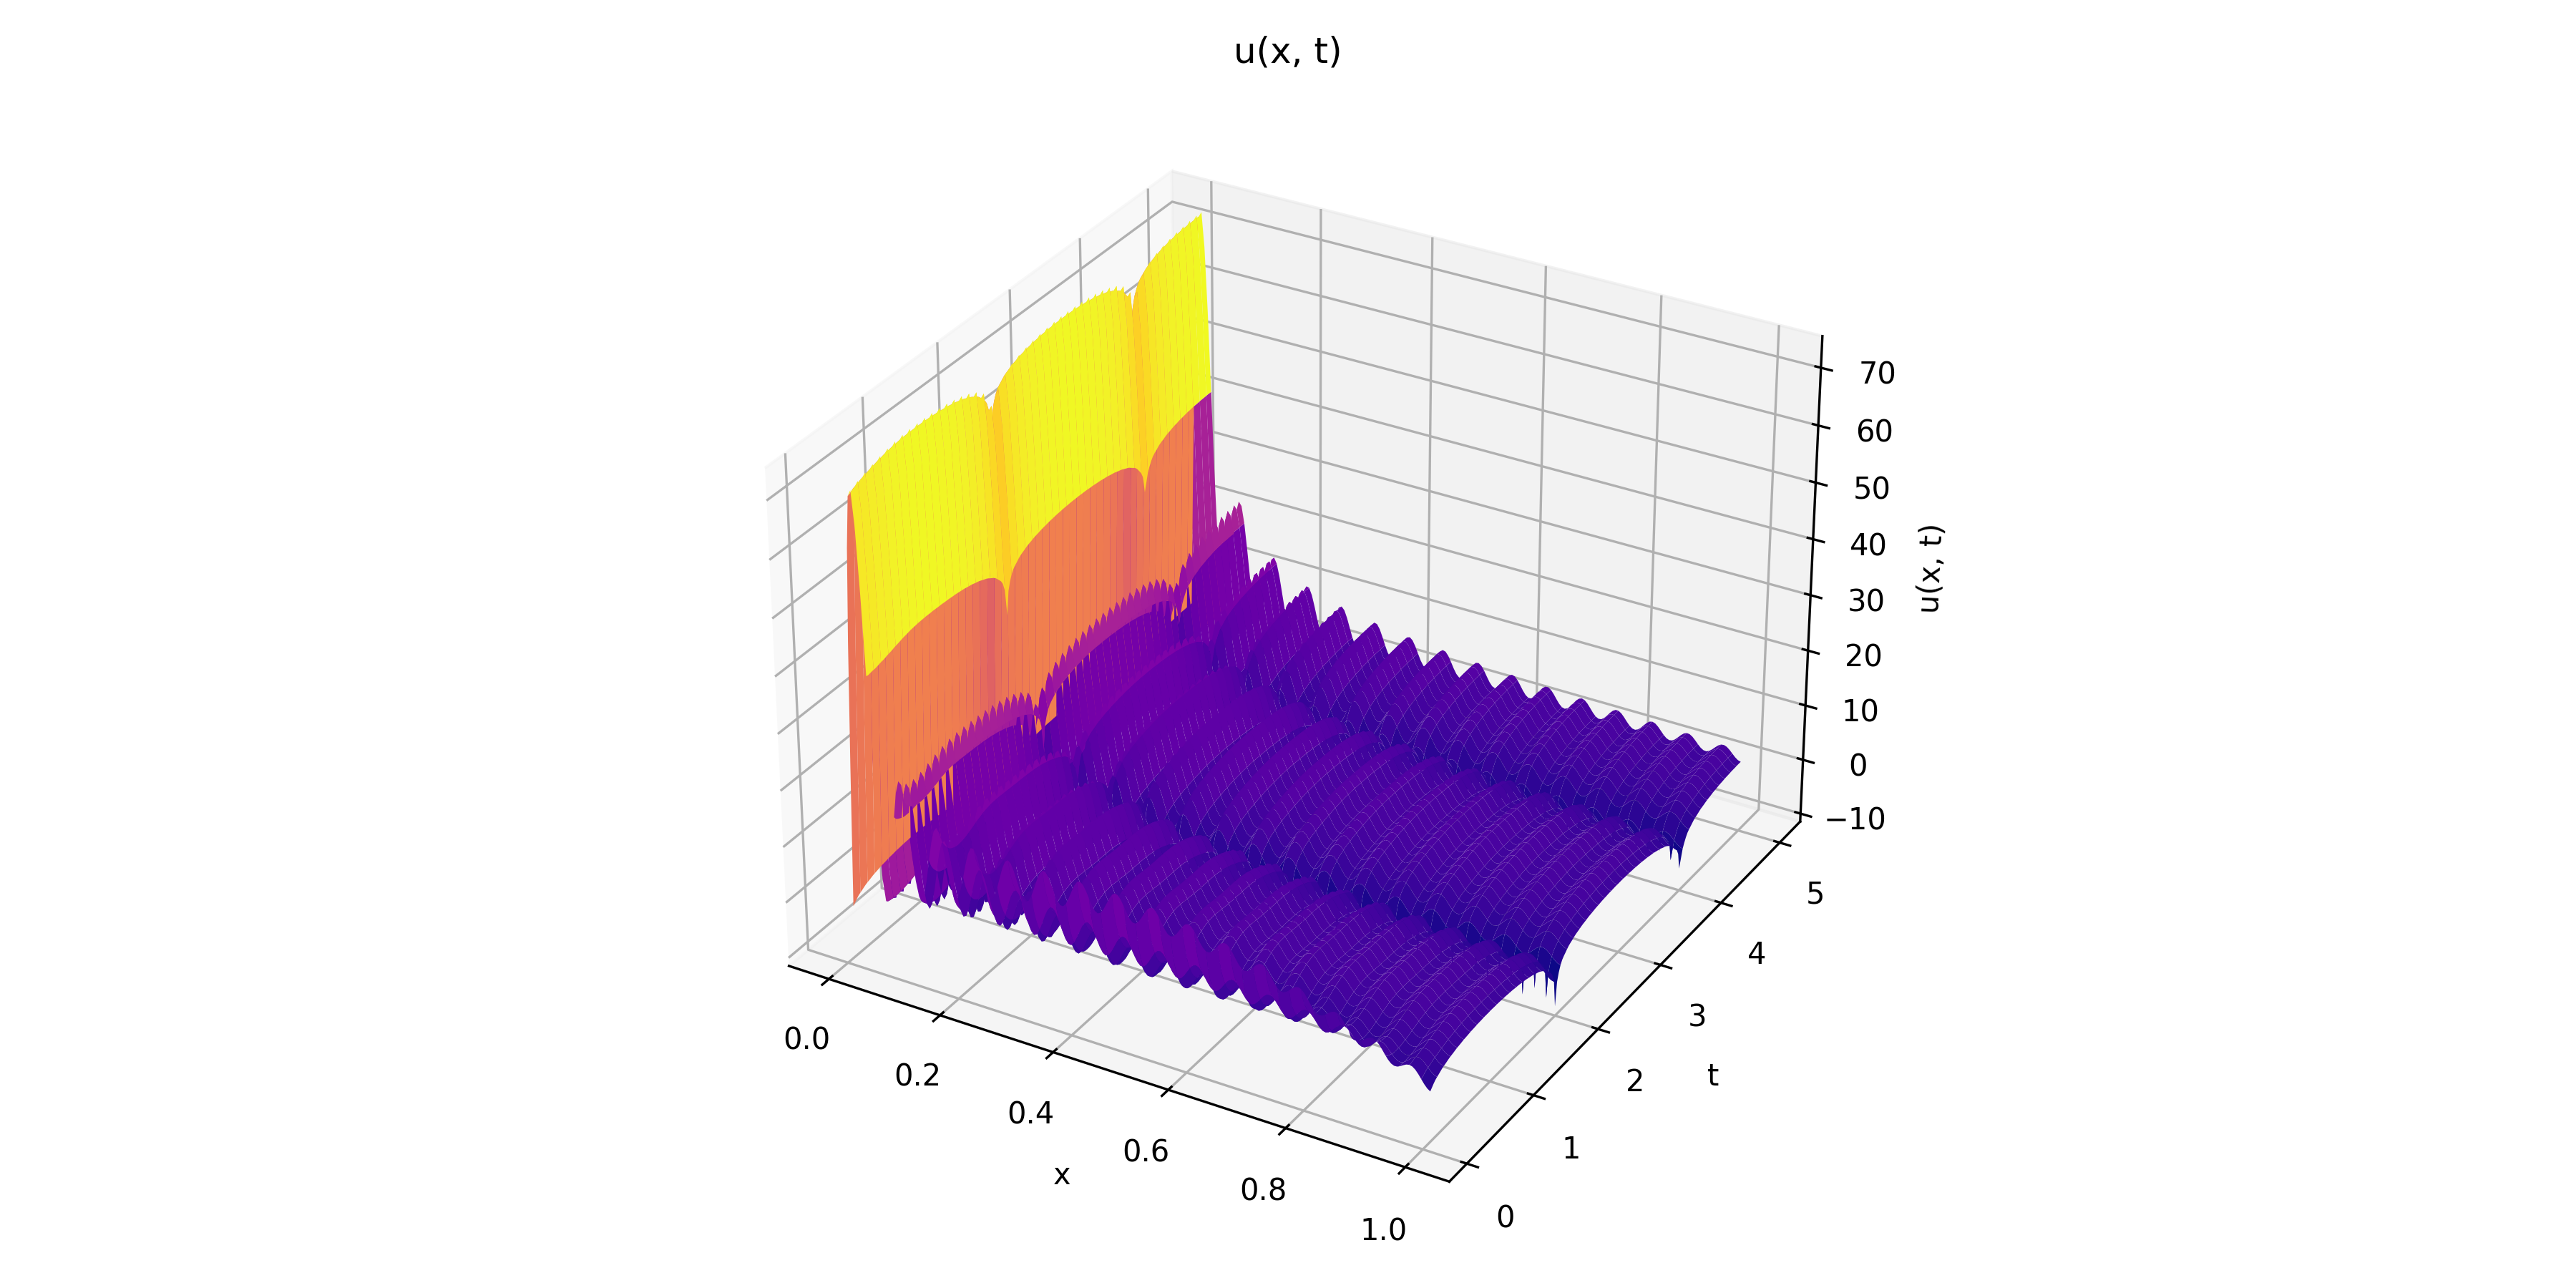
\includegraphics[width=0.8\textwidth]{../graph2.png}
    \caption{График функции $u(x,t)$, построенный по приближённой сумме ряда}
\end{figure}

\section{Визуализация 3}
$$u = \sum_{k=1}^{\infty}X_k T_k = \sum_{k=1}^{\infty} \frac{2l cos(\pi k)}{(\pi k)^2}cos(\frac{\pi k t}{l})cos(\frac{\pi k x}{l}) - \frac{t+1}{l}x^2 + tx$$
\textbf{Ниже приведен код на языке Python, который изображает график данной функции}
\begin{lstlisting}
  import numpy as np
import matplotlib.pyplot as plt
from mpl_toolkits.mplot3d import Axes3D

l = 1
N = 100 
x = np.linspace(0, l, 200)
t = np.linspace(0, 5, 200)
X, T = np.meshgrid(x, t)

U = np.zeros_like(X)

for k in range(1, N + 1):
    coef = (2 * l * np.cos(np.pi * k)) / ((np.pi * k)**2)
    U += coef * np.cos(np.pi * k * T / l) * np.cos(np.pi * k * X / l)

U += -((T + 1) / l) * X**2 + T * X

fig = plt.figure(figsize=(12, 6))
ax = fig.add_subplot(111, projection='3d')
ax.plot_surface(X, T, U, cmap='inferno')

ax.set_title("u(x, t)")
ax.set_xlabel("x")
ax.set_ylabel("t")
ax.set_zlabel("u(x, t)")

plt.tight_layout()
plt.savefig("graph3.png", dpi=300)
plt.show()

\end{lstlisting}
\begin{figure}[H]
    \centering
    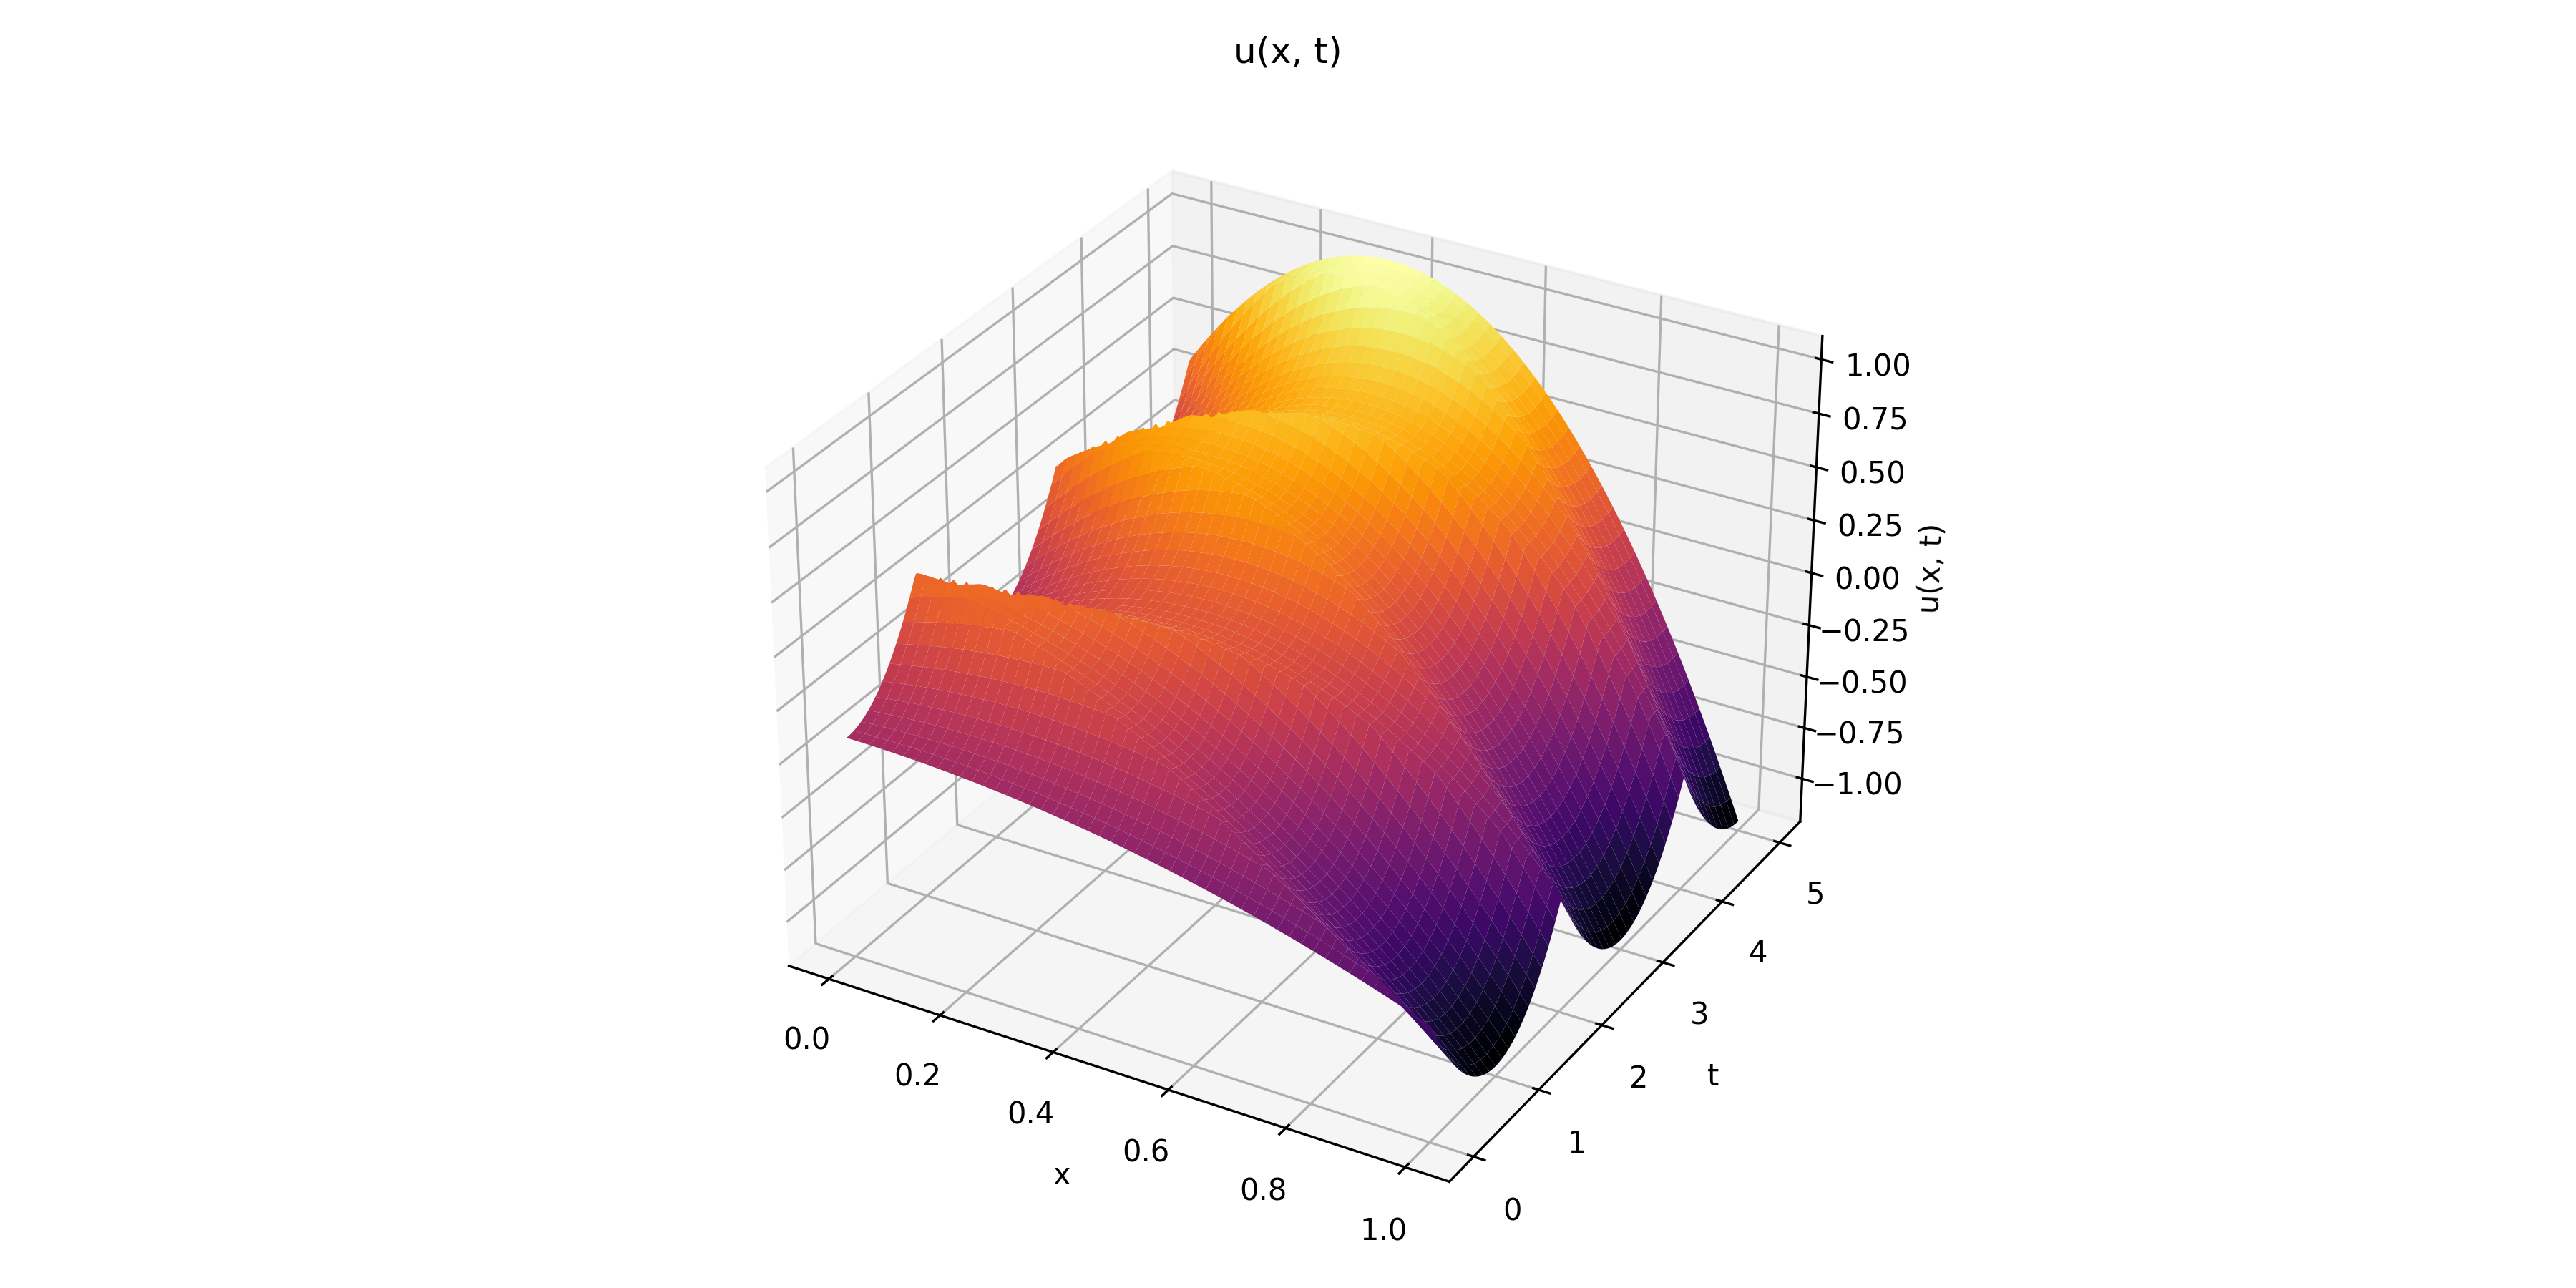
\includegraphics[width=0.8\textwidth]{../graph3.png}
    \caption{График функции $u(x,t)$, построенный по приближённой сумме ряда}
\end{figure}

\end{document}
